\documentclass[1p]{elsarticle_modified}
%\bibliographystyle{elsarticle-num}

%\usepackage[colorlinks]{hyperref}
%\usepackage{abbrmath_seonhwa} %\Abb, \Ascr, \Acal ,\Abf, \Afrak
\usepackage{amsfonts}
\usepackage{amssymb}
\usepackage{amsmath}
\usepackage{amsthm}
\usepackage{scalefnt}
\usepackage{amsbsy}
\usepackage{kotex}
\usepackage{caption}
\usepackage{subfig}
\usepackage{color}
\usepackage{graphicx}
\usepackage{xcolor} %% white, black, red, green, blue, cyan, magenta, yellow
\usepackage{float}
\usepackage{setspace}
\usepackage{hyperref}

\usepackage{tikz}
\usetikzlibrary{arrows}

\usepackage{multirow}
\usepackage{array} % fixed length table
\usepackage{hhline}

%%%%%%%%%%%%%%%%%%%%%
\makeatletter
\renewcommand*\env@matrix[1][\arraystretch]{%
	\edef\arraystretch{#1}%
	\hskip -\arraycolsep
	\let\@ifnextchar\new@ifnextchar
	\array{*\c@MaxMatrixCols c}}
\makeatother %https://tex.stackexchange.com/questions/14071/how-can-i-increase-the-line-spacing-in-a-matrix
%%%%%%%%%%%%%%%

\usepackage[normalem]{ulem}

\newcommand{\msout}[1]{\ifmmode\text{\sout{\ensuremath{#1}}}\else\sout{#1}\fi}
%SOURCE: \msout is \stkout macro in https://tex.stackexchange.com/questions/20609/strikeout-in-math-mode

\newcommand{\cancel}[1]{
	\ifmmode
	{\color{red}\msout{#1}}
	\else
	{\color{red}\sout{#1}}
	\fi
}

\newcommand{\add}[1]{
	{\color{blue}\uwave{#1}}
}

\newcommand{\replace}[2]{
	\ifmmode
	{\color{red}\msout{#1}}{\color{blue}\uwave{#2}}
	\else
	{\color{red}\sout{#1}}{\color{blue}\uwave{#2}}
	\fi
}

\newcommand{\Sol}{\mathcal{S}} %segment
\newcommand{\D}{D} %diagram
\newcommand{\A}{\mathcal{A}} %arc


%%%%%%%%%%%%%%%%%%%%%%%%%%%%%5 test

\def\sl{\operatorname{\textup{SL}}(2,\Cbb)}
\def\psl{\operatorname{\textup{PSL}}(2,\Cbb)}
\def\quan{\mkern 1mu \triangleright \mkern 1mu}

\theoremstyle{definition}
\newtheorem{thm}{Theorem}[section]
\newtheorem{prop}[thm]{Proposition}
\newtheorem{lem}[thm]{Lemma}
\newtheorem{ques}[thm]{Question}
\newtheorem{cor}[thm]{Corollary}
\newtheorem{defn}[thm]{Definition}
\newtheorem{exam}[thm]{Example}
\newtheorem{rmk}[thm]{Remark}
\newtheorem{alg}[thm]{Algorithm}

\newcommand{\I}{\sqrt{-1}}
\begin{document}

%\begin{frontmatter}
%
%\title{Boundary parabolic representations of knots up to 8 crossings}
%
%%% Group authors per affiliation:
%\author{Yunhi Cho} 
%\address{Department of Mathematics, University of Seoul, Seoul, Korea}
%\ead{yhcho@uos.ac.kr}
%
%
%\author{Seonhwa Kim} %\fnref{s_kim}}
%\address{Center for Geometry and Physics, Institute for Basic Science, Pohang, 37673, Korea}
%\ead{ryeona17@ibs.re.kr}
%
%\author{Hyuk Kim}
%\address{Department of Mathematical Sciences, Seoul National University, Seoul 08826, Korea}
%\ead{hyukkim@snu.ac.kr}
%
%\author{Seokbeom Yoon}
%\address{Department of Mathematical Sciences, Seoul National University, Seoul, 08826,  Korea}
%\ead{sbyoon15@snu.ac.kr}
%
%\begin{abstract}
%We find all boundary parabolic representation of knots up to 8 crossings.
%
%\end{abstract}
%\begin{keyword}
%    \MSC[2010] 57M25 
%\end{keyword}
%
%\end{frontmatter}

%\linenumbers
%\tableofcontents
%
\newcommand\colored[1]{\textcolor{white}{\rule[-0.35ex]{0.8em}{1.4ex}}\kern-0.8em\color{red} #1}%
%\newcommand\colored[1]{\textcolor{white}{ #1}\kern-2.17ex	\textcolor{white}{ #1}\kern-1.81ex	\textcolor{white}{ #1}\kern-2.15ex\color{red}#1	}

{\Large $\underline{11n_{10}~(K11n_{10})}$}

\setlength{\tabcolsep}{10pt}
\renewcommand{\arraystretch}{1.6}
\vspace{1cm}\begin{tabular}{m{100pt}>{\centering\arraybackslash}m{274pt}}
\multirow{5}{120pt}{
	\centering
	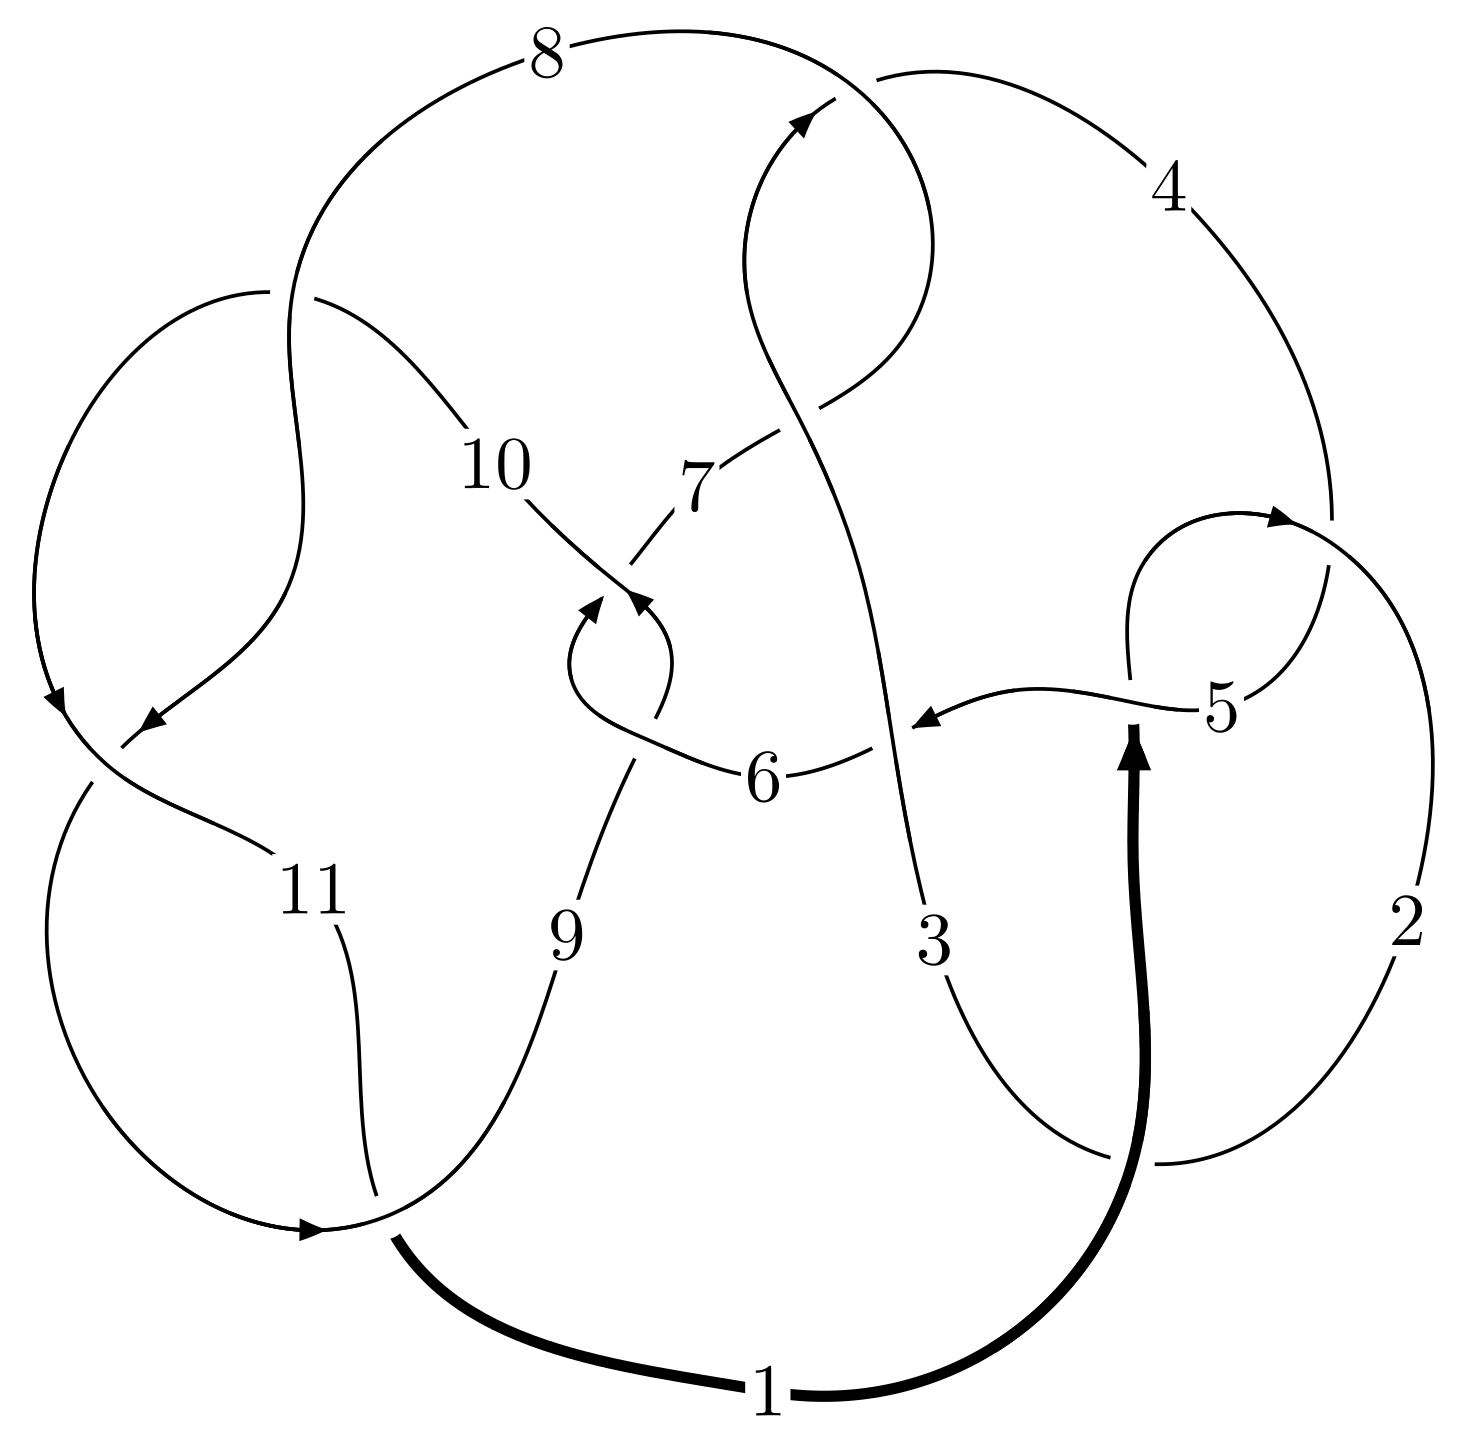
\includegraphics[width=112pt]{../../../GIT/diagram.site/Diagrams/png/626_11n_10.png}\\
\ \ \ A knot diagram\footnotemark}&
\allowdisplaybreaks
\textbf{Linearized knot diagam} \\
\cline{2-2}
 &
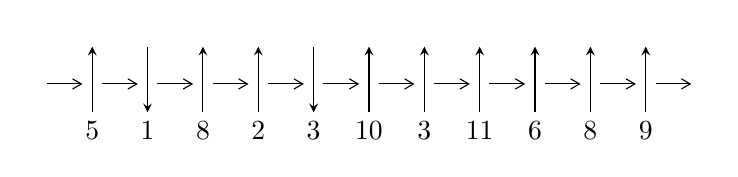
\begin{tikzpicture}[x=20pt, y=17pt]
	% nodes
	\node (C0) at (0, 0) {};
	\node (C1) at (1, 0) {};
	\node (C1U) at (1, +1) {};
	\node (C1D) at (1, -1) {5};

	\node (C2) at (2, 0) {};
	\node (C2U) at (2, +1) {};
	\node (C2D) at (2, -1) {1};

	\node (C3) at (3, 0) {};
	\node (C3U) at (3, +1) {};
	\node (C3D) at (3, -1) {8};

	\node (C4) at (4, 0) {};
	\node (C4U) at (4, +1) {};
	\node (C4D) at (4, -1) {2};

	\node (C5) at (5, 0) {};
	\node (C5U) at (5, +1) {};
	\node (C5D) at (5, -1) {3};

	\node (C6) at (6, 0) {};
	\node (C6U) at (6, +1) {};
	\node (C6D) at (6, -1) {10};

	\node (C7) at (7, 0) {};
	\node (C7U) at (7, +1) {};
	\node (C7D) at (7, -1) {3};

	\node (C8) at (8, 0) {};
	\node (C8U) at (8, +1) {};
	\node (C8D) at (8, -1) {11};

	\node (C9) at (9, 0) {};
	\node (C9U) at (9, +1) {};
	\node (C9D) at (9, -1) {6};

	\node (C10) at (10, 0) {};
	\node (C10U) at (10, +1) {};
	\node (C10D) at (10, -1) {8};

	\node (C11) at (11, 0) {};
	\node (C11U) at (11, +1) {};
	\node (C11D) at (11, -1) {9};
	\node (C12) at (12, 0) {};

	% arrows
	\draw[->,>={angle 60}]
	(C0) edge (C1) (C1) edge (C2) (C2) edge (C3) (C3) edge (C4) (C4) edge (C5) (C5) edge (C6) (C6) edge (C7) (C7) edge (C8) (C8) edge (C9) (C9) edge (C10) (C10) edge (C11) (C11) edge (C12) ;	\draw[->,>=stealth]
	(C1D) edge (C1U) (C2U) edge (C2D) (C3D) edge (C3U) (C4D) edge (C4U) (C5U) edge (C5D) (C6D) edge (C6U) (C7D) edge (C7U) (C8D) edge (C8U) (C9D) edge (C9U) (C10D) edge (C10U) (C11D) edge (C11U) ;
	\end{tikzpicture} \\
\hhline{~~} \\& 
\textbf{Solving Sequence} \\ \cline{2-2} 
 &
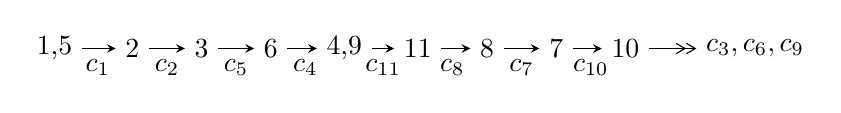
\begin{tikzpicture}[x=25pt, y=7pt]
	% node
	\node (A0) at (-1/8, 0) {1,5};
	\node (A1) at (1, 0) {2};
	\node (A2) at (2, 0) {3};
	\node (A3) at (3, 0) {6};
	\node (A4) at (65/16, 0) {4,9};
	\node (A5) at (41/8, 0) {11};
	\node (A6) at (49/8, 0) {8};
	\node (A7) at (57/8, 0) {7};
	\node (A8) at (65/8, 0) {10};
	\node (C1) at (1/2, -1) {$c_{1}$};
	\node (C2) at (3/2, -1) {$c_{2}$};
	\node (C3) at (5/2, -1) {$c_{5}$};
	\node (C4) at (7/2, -1) {$c_{4}$};
	\node (C5) at (37/8, -1) {$c_{11}$};
	\node (C6) at (45/8, -1) {$c_{8}$};
	\node (C7) at (53/8, -1) {$c_{7}$};
	\node (C8) at (61/8, -1) {$c_{10}$};
	\node (A9) at (10, 0) {$c_{3},c_{6},c_{9}$};

	% edge
	\draw[->,>=stealth]	
	(A0) edge (A1) (A1) edge (A2) (A2) edge (A3) (A3) edge (A4) (A4) edge (A5) (A5) edge (A6) (A6) edge (A7) (A7) edge (A8) ;
	\draw[->>,>={angle 60}]	
	(A8) edge (A9);
\end{tikzpicture} \\ 

\end{tabular} \\

\footnotetext{
The image of knot diagram is generated by the software ``\textbf{Draw programme}" developed by Andrew Bartholomew(\url{http://www.layer8.co.uk/maths/draw/index.htm\#Running-draw}), where we modified some parts for our purpose(\url{https://github.com/CATsTAILs/LinksPainter}).
}\phantom \\ \newline 
\centering \textbf{Ideals for irreducible components\footnotemark of $X_{\text{par}}$} 
 
\begin{align*}
I^u_{1}&=\langle 
8787304659 u^{35}-103954721318 u^{34}+\cdots+475816620046 b-403612228244,\\
\phantom{I^u_{1}}&\phantom{= \langle  }-377185205844 u^{35}+1123281301673 u^{34}+\cdots+475816620046 a-327197785091,\\
\phantom{I^u_{1}}&\phantom{= \langle  }u^{36}-3 u^{35}+\cdots+2 u+1\rangle \\
I^u_{2}&=\langle 
- a u+b+u,\;a^2- a u-3 a+2,\;u^2+u+1\rangle \\
\\
\end{align*}
\raggedright * 2 irreducible components of $\dim_{\mathbb{C}}=0$, with total 40 representations.\\
\footnotetext{All coefficients of polynomials are rational numbers. But the coefficients are sometimes approximated in decimal forms when there is not enough margin.}
\newpage
\renewcommand{\arraystretch}{1}
\centering \section*{I. $I^u_{1}= \langle 8.79\times10^{9} u^{35}-1.04\times10^{11} u^{34}+\cdots+4.76\times10^{11} b-4.04\times10^{11},\;-3.77\times10^{11} u^{35}+1.12\times10^{12} u^{34}+\cdots+4.76\times10^{11} a-3.27\times10^{11},\;u^{36}-3 u^{35}+\cdots+2 u+1 \rangle$}
\flushleft \textbf{(i) Arc colorings}\\
\begin{tabular}{m{7pt} m{180pt} m{7pt} m{180pt} }
\flushright $a_{1}=$&$\begin{pmatrix}1\\0\end{pmatrix}$ \\
\flushright $a_{5}=$&$\begin{pmatrix}0\\u\end{pmatrix}$ \\
\flushright $a_{2}=$&$\begin{pmatrix}1\\- u^2\end{pmatrix}$ \\
\flushright $a_{3}=$&$\begin{pmatrix}u^2+1\\- u^2\end{pmatrix}$ \\
\flushright $a_{6}=$&$\begin{pmatrix}- u^5-2 u^3- u\\u^5+u^3+u\end{pmatrix}$ \\
\flushright $a_{4}=$&$\begin{pmatrix}- u\\u^3+u\end{pmatrix}$ \\
\flushright $a_{9}=$&$\begin{pmatrix}0.792711 u^{35}-2.36074 u^{34}+\cdots-7.92555 u+0.687655\\-0.0184678 u^{35}+0.218476 u^{34}+\cdots+2.06332 u+0.848252\end{pmatrix}$ \\
\flushright $a_{11}=$&$\begin{pmatrix}1.81069 u^{35}-3.83855 u^{34}+\cdots-5.73449 u+0.597631\\-1.42613 u^{35}+4.12609 u^{34}+\cdots+4.24671 u+1.60699\end{pmatrix}$ \\
\flushright $a_{8}=$&$\begin{pmatrix}-1.48252 u^{35}+2.76287 u^{34}+\cdots+0.445446 u+2.16820\\1.68468 u^{35}-5.18476 u^{34}+\cdots-5.13324 u-1.48252\end{pmatrix}$ \\
\flushright $a_{7}=$&$\begin{pmatrix}-3.01339 u^{35}+5.80035 u^{34}+\cdots+3.96183 u+2.75504\\3.24321 u^{35}-9.22497 u^{34}+\cdots-6.94504 u-2.40225\end{pmatrix}$ \\
\flushright $a_{10}=$&$\begin{pmatrix}-0.224280 u^{35}-0.364289 u^{34}+\cdots-6.62538 u+1.26123\\1.20451 u^{35}-3.50438 u^{34}+\cdots-0.486823 u-0.427974\end{pmatrix}$\\ \flushright $a_{10}=$&$\begin{pmatrix}-0.224280 u^{35}-0.364289 u^{34}+\cdots-6.62538 u+1.26123\\1.20451 u^{35}-3.50438 u^{34}+\cdots-0.486823 u-0.427974\end{pmatrix}$\\&\end{tabular}
\flushleft \textbf{(ii) Obstruction class $= -1$}\\~\\
\flushleft \textbf{(iii) Cusp Shapes $= \frac{132200220423}{475816620046} u^{35}-\frac{80372153223}{237908310023} u^{34}+\cdots-\frac{2105018315229}{475816620046} u+\frac{2668832099181}{237908310023}$}\\~\\
\newpage\renewcommand{\arraystretch}{1}
\flushleft \textbf{(iv) u-Polynomials at the component}\newline \\
\begin{tabular}{m{50pt}|m{274pt}}
Crossings & \hspace{64pt}u-Polynomials at each crossing \\
\hline $$\begin{aligned}c_{1},c_{4}\end{aligned}$$&$\begin{aligned}
&u^{36}+3 u^{35}+\cdots-2 u+1
\end{aligned}$\\
\hline $$\begin{aligned}c_{2}\end{aligned}$$&$\begin{aligned}
&u^{36}+19 u^{35}+\cdots-30 u+1
\end{aligned}$\\
\hline $$\begin{aligned}c_{3},c_{7}\end{aligned}$$&$\begin{aligned}
&u^{36}+3 u^{35}+\cdots-80 u+16
\end{aligned}$\\
\hline $$\begin{aligned}c_{5}\end{aligned}$$&$\begin{aligned}
&u^{36}-3 u^{35}+\cdots-552 u+97
\end{aligned}$\\
\hline $$\begin{aligned}c_{6},c_{9}\end{aligned}$$&$\begin{aligned}
&u^{36}-3 u^{35}+\cdots+7 u^2-1
\end{aligned}$\\
\hline $$\begin{aligned}c_{8},c_{10},c_{11}\end{aligned}$$&$\begin{aligned}
&u^{36}+3 u^{35}+\cdots+8 u-1
\end{aligned}$\\
\hline
\end{tabular}\\~\\
\newpage\renewcommand{\arraystretch}{1}
\flushleft \textbf{(v) Riley Polynomials at the component}\newline \\
\begin{tabular}{m{50pt}|m{274pt}}
Crossings & \hspace{64pt}Riley Polynomials at each crossing \\
\hline $$\begin{aligned}c_{1},c_{4}\end{aligned}$$&$\begin{aligned}
&y^{36}+19 y^{35}+\cdots-30 y+1
\end{aligned}$\\
\hline $$\begin{aligned}c_{2}\end{aligned}$$&$\begin{aligned}
&y^{36}- y^{35}+\cdots-1390 y+1
\end{aligned}$\\
\hline $$\begin{aligned}c_{3},c_{7}\end{aligned}$$&$\begin{aligned}
&y^{36}+25 y^{35}+\cdots+384 y+256
\end{aligned}$\\
\hline $$\begin{aligned}c_{5}\end{aligned}$$&$\begin{aligned}
&y^{36}-21 y^{35}+\cdots-232342 y+9409
\end{aligned}$\\
\hline $$\begin{aligned}c_{6},c_{9}\end{aligned}$$&$\begin{aligned}
&y^{36}-9 y^{35}+\cdots-14 y+1
\end{aligned}$\\
\hline $$\begin{aligned}c_{8},c_{10},c_{11}\end{aligned}$$&$\begin{aligned}
&y^{36}-29 y^{35}+\cdots-14 y+1
\end{aligned}$\\
\hline
\end{tabular}\\~\\
\newpage\flushleft \textbf{(vi) Complex Volumes and Cusp Shapes}
$$\begin{array}{c|c|c}  
\text{Solutions to }I^u_{1}& \I (\text{vol} + \sqrt{-1}CS) & \text{Cusp shape}\\
 \hline 
\begin{aligned}
u &= \phantom{-}0.941953 + 0.318856 I \\
a &= \phantom{-}1.90171 - 0.06813 I \\
b &= -1.330950 + 0.428412 I\end{aligned}
 & \phantom{-}1.25207 - 7.91102 I & \phantom{-}10.72087 + 4.98053 I \\ \hline\begin{aligned}
u &= \phantom{-}0.941953 - 0.318856 I \\
a &= \phantom{-}1.90171 + 0.06813 I \\
b &= -1.330950 - 0.428412 I\end{aligned}
 & \phantom{-}1.25207 + 7.91102 I & \phantom{-}10.72087 - 4.98053 I \\ \hline\begin{aligned}
u &= -0.578922 + 0.827435 I \\
a &= \phantom{-}0.466797 - 0.077681 I \\
b &= \phantom{-}0.222633 - 0.152510 I\end{aligned}
 & \phantom{-}0.57502 - 2.28935 I & \phantom{-}0.59495 + 6.49088 I \\ \hline\begin{aligned}
u &= -0.578922 - 0.827435 I \\
a &= \phantom{-}0.466797 + 0.077681 I \\
b &= \phantom{-}0.222633 + 0.152510 I\end{aligned}
 & \phantom{-}0.57502 + 2.28935 I & \phantom{-}0.59495 - 6.49088 I \\ \hline\begin{aligned}
u &= -0.462897 + 0.928342 I \\
a &= \phantom{-}0.53466 - 3.01700 I \\
b &= \phantom{-}0.991548 - 0.131048 I\end{aligned}
 & \phantom{-}1.36980 - 2.39965 I & \phantom{-}20.4935 - 7.9827 I \\ \hline\begin{aligned}
u &= -0.462897 - 0.928342 I \\
a &= \phantom{-}0.53466 + 3.01700 I \\
b &= \phantom{-}0.991548 + 0.131048 I\end{aligned}
 & \phantom{-}1.36980 + 2.39965 I & \phantom{-}20.4935 + 7.9827 I \\ \hline\begin{aligned}
u &= -0.958743\phantom{ +0.000000I} \\
a &= \phantom{-}1.33018\phantom{ +0.000000I} \\
b &= -1.21120\phantom{ +0.000000I}\end{aligned}
 & \phantom{-}5.21748\phantom{ +0.000000I} & \phantom{-}18.9740\phantom{ +0.000000I} \\ \hline\begin{aligned}
u &= \phantom{-}0.390666 + 0.829574 I \\
a &= \phantom{-}1.76642 - 1.65948 I \\
b &= -1.64687 - 0.04349 I\end{aligned}
 & \phantom{-}8.65750 + 1.68497 I & \phantom{-}4.45327 + 6.62838 I \\ \hline\begin{aligned}
u &= \phantom{-}0.390666 - 0.829574 I \\
a &= \phantom{-}1.76642 + 1.65948 I \\
b &= -1.64687 + 0.04349 I\end{aligned}
 & \phantom{-}8.65750 - 1.68497 I & \phantom{-}4.45327 - 6.62838 I \\ \hline\begin{aligned}
u &= -0.352390 + 1.060720 I \\
a &= \phantom{-}0.288497 - 0.584924 I \\
b &= -0.100145 - 0.439780 I\end{aligned}
 & -1.38239 - 2.67848 I & \phantom{-}3.33680 + 4.36497 I\\
 \hline 
 \end{array}$$\newpage$$\begin{array}{c|c|c}  
\text{Solutions to }I^u_{1}& \I (\text{vol} + \sqrt{-1}CS) & \text{Cusp shape}\\
 \hline 
\begin{aligned}
u &= -0.352390 - 1.060720 I \\
a &= \phantom{-}0.288497 + 0.584924 I \\
b &= -0.100145 + 0.439780 I\end{aligned}
 & -1.38239 + 2.67848 I & \phantom{-}3.33680 - 4.36497 I \\ \hline\begin{aligned}
u &= \phantom{-}0.836718 + 0.162292 I \\
a &= \phantom{-}0.139245 + 0.541740 I \\
b &= \phantom{-}0.055080 - 0.891815 I\end{aligned}
 & -3.08076 - 3.16131 I & \phantom{-}6.74911 + 2.73736 I \\ \hline\begin{aligned}
u &= \phantom{-}0.836718 - 0.162292 I \\
a &= \phantom{-}0.139245 - 0.541740 I \\
b &= \phantom{-}0.055080 + 0.891815 I\end{aligned}
 & -3.08076 + 3.16131 I & \phantom{-}6.74911 - 2.73736 I \\ \hline\begin{aligned}
u &= -0.429143 + 0.677623 I \\
a &= -2.71700 + 1.40590 I \\
b &= \phantom{-}1.153580 + 0.008712 I\end{aligned}
 & \phantom{-}2.13722 - 1.37641 I & \phantom{-}5.40609 + 5.14317 I \\ \hline\begin{aligned}
u &= -0.429143 - 0.677623 I \\
a &= -2.71700 - 1.40590 I \\
b &= \phantom{-}1.153580 - 0.008712 I\end{aligned}
 & \phantom{-}2.13722 + 1.37641 I & \phantom{-}5.40609 - 5.14317 I \\ \hline\begin{aligned}
u &= \phantom{-}0.418004 + 1.152660 I \\
a &= -0.330548 + 0.337367 I \\
b &= \phantom{-}1.222910 - 0.619715 I\end{aligned}
 & -2.79850 + 2.36350 I & \phantom{-}5.53508 - 2.60014 I \\ \hline\begin{aligned}
u &= \phantom{-}0.418004 - 1.152660 I \\
a &= -0.330548 - 0.337367 I \\
b &= \phantom{-}1.222910 + 0.619715 I\end{aligned}
 & -2.79850 - 2.36350 I & \phantom{-}5.53508 + 2.60014 I \\ \hline\begin{aligned}
u &= -0.917196 + 0.828372 I \\
a &= \phantom{-}1.65210 + 0.46733 I \\
b &= -1.186090 + 0.089252 I\end{aligned}
 & \phantom{-}4.37030 - 3.28706 I & \phantom{-}16.3776 + 6.4044 I \\ \hline\begin{aligned}
u &= -0.917196 - 0.828372 I \\
a &= \phantom{-}1.65210 - 0.46733 I \\
b &= -1.186090 - 0.089252 I\end{aligned}
 & \phantom{-}4.37030 + 3.28706 I & \phantom{-}16.3776 - 6.4044 I \\ \hline\begin{aligned}
u &= \phantom{-}0.482228 + 1.156400 I \\
a &= -1.53682 + 1.54127 I \\
b &= \phantom{-}1.42553 + 0.42860 I\end{aligned}
 & -2.33330 + 5.78583 I & \phantom{-}6.12375 - 4.54634 I\\
 \hline 
 \end{array}$$\newpage$$\begin{array}{c|c|c}  
\text{Solutions to }I^u_{1}& \I (\text{vol} + \sqrt{-1}CS) & \text{Cusp shape}\\
 \hline 
\begin{aligned}
u &= \phantom{-}0.482228 - 1.156400 I \\
a &= -1.53682 - 1.54127 I \\
b &= \phantom{-}1.42553 - 0.42860 I\end{aligned}
 & -2.33330 - 5.78583 I & \phantom{-}6.12375 + 4.54634 I \\ \hline\begin{aligned}
u &= \phantom{-}0.355005 + 1.235300 I \\
a &= \phantom{-}0.736458 - 0.433010 I \\
b &= -0.170722 - 0.941275 I\end{aligned}
 & -7.38923 + 0.84480 I & \phantom{-}2.27275 - 0.94603 I \\ \hline\begin{aligned}
u &= \phantom{-}0.355005 - 1.235300 I \\
a &= \phantom{-}0.736458 + 0.433010 I \\
b &= -0.170722 + 0.941275 I\end{aligned}
 & -7.38923 - 0.84480 I & \phantom{-}2.27275 + 0.94603 I \\ \hline\begin{aligned}
u &= \phantom{-}0.528429 + 1.198920 I \\
a &= -0.764889 + 0.265751 I \\
b &= \phantom{-}0.118707 + 1.039180 I\end{aligned}
 & -6.16236 + 8.15772 I & \phantom{-}4.34763 - 5.90259 I \\ \hline\begin{aligned}
u &= \phantom{-}0.528429 - 1.198920 I \\
a &= -0.764889 - 0.265751 I \\
b &= \phantom{-}0.118707 - 1.039180 I\end{aligned}
 & -6.16236 - 8.15772 I & \phantom{-}4.34763 + 5.90259 I \\ \hline\begin{aligned}
u &= \phantom{-}0.191310 + 1.304130 I \\
a &= \phantom{-}0.267608 + 0.045241 I \\
b &= -1.157150 + 0.494867 I\end{aligned}
 & -4.36779 - 4.25736 I & \phantom{-}4.95189 + 4.14577 I \\ \hline\begin{aligned}
u &= \phantom{-}0.191310 - 1.304130 I \\
a &= \phantom{-}0.267608 - 0.045241 I \\
b &= -1.157150 - 0.494867 I\end{aligned}
 & -4.36779 + 4.25736 I & \phantom{-}4.95189 - 4.14577 I \\ \hline\begin{aligned}
u &= \phantom{-}0.667019 + 0.112397 I \\
a &= -2.55104 - 0.08549 I \\
b &= \phantom{-}1.252170 - 0.381251 I\end{aligned}
 & \phantom{-}0.59829 - 1.41278 I & \phantom{-}9.58916 + 0.83279 I \\ \hline\begin{aligned}
u &= \phantom{-}0.667019 - 0.112397 I \\
a &= -2.55104 + 0.08549 I \\
b &= \phantom{-}1.252170 + 0.381251 I\end{aligned}
 & \phantom{-}0.59829 + 1.41278 I & \phantom{-}9.58916 - 0.83279 I \\ \hline\begin{aligned}
u &= -0.076900 + 0.656111 I \\
a &= -0.25086 + 1.59937 I \\
b &= \phantom{-}0.571894 + 0.426603 I\end{aligned}
 & \phantom{-}0.502483 + 0.088457 I & \phantom{-}8.19922 - 0.63999 I\\
 \hline 
 \end{array}$$\newpage$$\begin{array}{c|c|c}  
\text{Solutions to }I^u_{1}& \I (\text{vol} + \sqrt{-1}CS) & \text{Cusp shape}\\
 \hline 
\begin{aligned}
u &= -0.076900 - 0.656111 I \\
a &= -0.25086 - 1.59937 I \\
b &= \phantom{-}0.571894 - 0.426603 I\end{aligned}
 & \phantom{-}0.502483 - 0.088457 I & \phantom{-}8.19922 + 0.63999 I \\ \hline\begin{aligned}
u &= \phantom{-}0.616178 + 1.196580 I \\
a &= \phantom{-}1.49880 - 1.41745 I \\
b &= -1.39338 - 0.48591 I\end{aligned}
 & -1.43022 + 13.58250 I & \phantom{-}8.11529 - 8.04740 I \\ \hline\begin{aligned}
u &= \phantom{-}0.616178 - 1.196580 I \\
a &= \phantom{-}1.49880 + 1.41745 I \\
b &= -1.39338 + 0.48591 I\end{aligned}
 & -1.43022 - 13.58250 I & \phantom{-}8.11529 + 8.04740 I \\ \hline\begin{aligned}
u &= -0.548564 + 1.246830 I \\
a &= \phantom{-}0.708615 + 0.979572 I \\
b &= -1.132080 + 0.226075 I\end{aligned}
 & \phantom{-}1.52668 - 5.32517 I & \phantom{-}10.19862 + 8.96318 I \\ \hline\begin{aligned}
u &= -0.548564 - 1.246830 I \\
a &= \phantom{-}0.708615 - 0.979572 I \\
b &= -1.132080 - 0.226075 I\end{aligned}
 & \phantom{-}1.52668 + 5.32517 I & \phantom{-}10.19862 - 8.96318 I \\ \hline\begin{aligned}
u &= -0.164250\phantom{ +0.000000I} \\
a &= \phantom{-}3.05031\phantom{ +0.000000I} \\
b &= \phantom{-}0.417861\phantom{ +0.000000I}\end{aligned}
 & \phantom{-}0.823260\phantom{ +0.000000I} & \phantom{-}12.0950\phantom{ +0.000000I}\\
 \hline 
 \end{array}$$\newpage\newpage\renewcommand{\arraystretch}{1}
\centering \section*{II. $I^u_{2}= \langle - a u+b+u,\;a^2- a u-3 a+2,\;u^2+u+1 \rangle$}
\flushleft \textbf{(i) Arc colorings}\\
\begin{tabular}{m{7pt} m{180pt} m{7pt} m{180pt} }
\flushright $a_{1}=$&$\begin{pmatrix}1\\0\end{pmatrix}$ \\
\flushright $a_{5}=$&$\begin{pmatrix}0\\u\end{pmatrix}$ \\
\flushright $a_{2}=$&$\begin{pmatrix}1\\u+1\end{pmatrix}$ \\
\flushright $a_{3}=$&$\begin{pmatrix}- u\\u+1\end{pmatrix}$ \\
\flushright $a_{6}=$&$\begin{pmatrix}-1\\0\end{pmatrix}$ \\
\flushright $a_{4}=$&$\begin{pmatrix}- u\\u+1\end{pmatrix}$ \\
\flushright $a_{9}=$&$\begin{pmatrix}a\\a u- u\end{pmatrix}$ \\
\flushright $a_{11}=$&$\begin{pmatrix}a u- a-2 u+1\\- a u+u+1\end{pmatrix}$ \\
\flushright $a_{8}=$&$\begin{pmatrix}- a- u\\- a u+u+1\end{pmatrix}$ \\
\flushright $a_{7}=$&$\begin{pmatrix}- a- u\\- a u+u+1\end{pmatrix}$ \\
\flushright $a_{10}=$&$\begin{pmatrix}a u+a- u\\a u- u\end{pmatrix}$\\ \flushright $a_{10}=$&$\begin{pmatrix}a u+a- u\\a u- u\end{pmatrix}$\\&\end{tabular}
\flushleft \textbf{(ii) Obstruction class $= 1$}\\~\\
\flushleft \textbf{(iii) Cusp Shapes $= 3 a u+6 a-2 u+10$}\\~\\
\newpage\renewcommand{\arraystretch}{1}
\flushleft \textbf{(iv) u-Polynomials at the component}\newline \\
\begin{tabular}{m{50pt}|m{274pt}}
Crossings & \hspace{64pt}u-Polynomials at each crossing \\
\hline $$\begin{aligned}c_{1},c_{2},c_{5}\end{aligned}$$&$\begin{aligned}
&(u^2+u+1)^2
\end{aligned}$\\
\hline $$\begin{aligned}c_{3},c_{7}\end{aligned}$$&$\begin{aligned}
&u^4
\end{aligned}$\\
\hline $$\begin{aligned}c_{4}\end{aligned}$$&$\begin{aligned}
&(u^2- u+1)^2
\end{aligned}$\\
\hline $$\begin{aligned}c_{6},c_{8}\end{aligned}$$&$\begin{aligned}
&(u^2- u-1)^2
\end{aligned}$\\
\hline $$\begin{aligned}c_{9},c_{10},c_{11}\end{aligned}$$&$\begin{aligned}
&(u^2+u-1)^2
\end{aligned}$\\
\hline
\end{tabular}\\~\\
\newpage\renewcommand{\arraystretch}{1}
\flushleft \textbf{(v) Riley Polynomials at the component}\newline \\
\begin{tabular}{m{50pt}|m{274pt}}
Crossings & \hspace{64pt}Riley Polynomials at each crossing \\
\hline $$\begin{aligned}c_{1},c_{2},c_{4}\\c_{5}\end{aligned}$$&$\begin{aligned}
&(y^2+y+1)^2
\end{aligned}$\\
\hline $$\begin{aligned}c_{3},c_{7}\end{aligned}$$&$\begin{aligned}
&y^4
\end{aligned}$\\
\hline $$\begin{aligned}c_{6},c_{8},c_{9}\\c_{10},c_{11}\end{aligned}$$&$\begin{aligned}
&(y^2-3 y+1)^2
\end{aligned}$\\
\hline
\end{tabular}\\~\\
\newpage\flushleft \textbf{(vi) Complex Volumes and Cusp Shapes}
$$\begin{array}{c|c|c}  
\text{Solutions to }I^u_{2}& \I (\text{vol} + \sqrt{-1}CS) & \text{Cusp shape}\\
 \hline 
\begin{aligned}
u &= -0.500000 + 0.866025 I \\
a &= \phantom{-}0.690983 - 0.535233 I \\
b &= \phantom{-}0.618034\phantom{ +0.000000I}\end{aligned}
 & \phantom{-}0.98696 - 2.02988 I & \phantom{-}15.5000 - 2.3454 I \\ \hline\begin{aligned}
u &= -0.500000 + 0.866025 I \\
a &= \phantom{-}1.80902 + 1.40126 I \\
b &= -1.61803\phantom{ +0.000000I}\end{aligned}
 & \phantom{-}8.88264 - 2.02988 I & \phantom{-}15.5000 + 9.2736 I \\ \hline\begin{aligned}
u &= -0.500000 - 0.866025 I \\
a &= \phantom{-}0.690983 + 0.535233 I \\
b &= \phantom{-}0.618034\phantom{ +0.000000I}\end{aligned}
 & \phantom{-}0.98696 + 2.02988 I & \phantom{-}15.5000 + 2.3454 I \\ \hline\begin{aligned}
u &= -0.500000 - 0.866025 I \\
a &= \phantom{-}1.80902 - 1.40126 I \\
b &= -1.61803\phantom{ +0.000000I}\end{aligned}
 & \phantom{-}8.88264 + 2.02988 I & \phantom{-}15.5000 - 9.2736 I\\
 \hline 
 \end{array}$$\newpage
\newpage\renewcommand{\arraystretch}{1}
\centering \section*{ III. u-Polynomials}
\begin{tabular}{m{50pt}|m{274pt}}
Crossings & \hspace{64pt}u-Polynomials at each crossing \\
\hline $$\begin{aligned}c_{1}\end{aligned}$$&$\begin{aligned}
&((u^2+u+1)^2)(u^{36}+3 u^{35}+\cdots-2 u+1)
\end{aligned}$\\
\hline $$\begin{aligned}c_{2}\end{aligned}$$&$\begin{aligned}
&((u^2+u+1)^2)(u^{36}+19 u^{35}+\cdots-30 u+1)
\end{aligned}$\\
\hline $$\begin{aligned}c_{3},c_{7}\end{aligned}$$&$\begin{aligned}
&u^4(u^{36}+3 u^{35}+\cdots-80 u+16)
\end{aligned}$\\
\hline $$\begin{aligned}c_{4}\end{aligned}$$&$\begin{aligned}
&((u^2- u+1)^2)(u^{36}+3 u^{35}+\cdots-2 u+1)
\end{aligned}$\\
\hline $$\begin{aligned}c_{5}\end{aligned}$$&$\begin{aligned}
&((u^2+u+1)^2)(u^{36}-3 u^{35}+\cdots-552 u+97)
\end{aligned}$\\
\hline $$\begin{aligned}c_{6}\end{aligned}$$&$\begin{aligned}
&((u^2- u-1)^2)(u^{36}-3 u^{35}+\cdots+7 u^2-1)
\end{aligned}$\\
\hline $$\begin{aligned}c_{8}\end{aligned}$$&$\begin{aligned}
&((u^2- u-1)^2)(u^{36}+3 u^{35}+\cdots+8 u-1)
\end{aligned}$\\
\hline $$\begin{aligned}c_{9}\end{aligned}$$&$\begin{aligned}
&((u^2+u-1)^2)(u^{36}-3 u^{35}+\cdots+7 u^2-1)
\end{aligned}$\\
\hline $$\begin{aligned}c_{10},c_{11}\end{aligned}$$&$\begin{aligned}
&((u^2+u-1)^2)(u^{36}+3 u^{35}+\cdots+8 u-1)
\end{aligned}$\\
\hline
\end{tabular}\newpage\renewcommand{\arraystretch}{1}
\centering \section*{ IV. Riley Polynomials}
\begin{tabular}{m{50pt}|m{274pt}}
Crossings & \hspace{64pt}Riley Polynomials at each crossing \\
\hline $$\begin{aligned}c_{1},c_{4}\end{aligned}$$&$\begin{aligned}
&((y^2+y+1)^2)(y^{36}+19 y^{35}+\cdots-30 y+1)
\end{aligned}$\\
\hline $$\begin{aligned}c_{2}\end{aligned}$$&$\begin{aligned}
&((y^2+y+1)^2)(y^{36}- y^{35}+\cdots-1390 y+1)
\end{aligned}$\\
\hline $$\begin{aligned}c_{3},c_{7}\end{aligned}$$&$\begin{aligned}
&y^4(y^{36}+25 y^{35}+\cdots+384 y+256)
\end{aligned}$\\
\hline $$\begin{aligned}c_{5}\end{aligned}$$&$\begin{aligned}
&((y^2+y+1)^2)(y^{36}-21 y^{35}+\cdots-232342 y+9409)
\end{aligned}$\\
\hline $$\begin{aligned}c_{6},c_{9}\end{aligned}$$&$\begin{aligned}
&((y^2-3 y+1)^2)(y^{36}-9 y^{35}+\cdots-14 y+1)
\end{aligned}$\\
\hline $$\begin{aligned}c_{8},c_{10},c_{11}\end{aligned}$$&$\begin{aligned}
&((y^2-3 y+1)^2)(y^{36}-29 y^{35}+\cdots-14 y+1)
\end{aligned}$\\
\hline
\end{tabular}
\vskip 2pc
\end{document}